% Created 2020-11-04 Wed 13:20
% Intended LaTeX compiler: pdflatex
\documentclass[presentation]{beamer}
\usepackage[utf8]{inputenc}
\usepackage[T1]{fontenc}
\usepackage{graphicx}
\usepackage{grffile}
\usepackage{longtable}
\usepackage{wrapfig}
\usepackage{rotating}
\usepackage[normalem]{ulem}
\usepackage{amsmath}
\usepackage{textcomp}
\usepackage{amssymb}
\usepackage{capt-of}
\usepackage{hyperref}
\usetheme{UoB}
\author{Mark Blyth}
\date{\textit{[2020-11-04 Wed]}}
\title{A year in the life of Mark}
\hypersetup{
 pdfauthor={Mark Blyth},
 pdftitle={A year in the life of Mark},
 pdfkeywords={},
 pdfsubject={},
 pdfcreator={Emacs 27.1 (Org mode 9.3)}, 
 pdflang={English}}
\begin{document}

\maketitle

\section{Background}
\label{sec:orgfa19b5e}
\begin{frame}[label={sec:org6723c6d}]{Today's agenda}
\begin{itemize}
\item \alert{A brief summary of things}
\end{itemize}
\vfill
\begin{itemize}
\item More CBC
\end{itemize}
\vfill
\begin{itemize}
\item Results so far
\end{itemize}
\vfill
\begin{itemize}
\item Current work
\end{itemize}
\vfill
\end{frame}

\section{A brief summary of things}
\label{sec:org34d4b2b}
\begin{frame}[label={sec:org9f9db64}]{What am I doing?}
\begin{itemize}
\item Neurons are interesting
\end{itemize}
\vfill
\begin{itemize}
\item Nonlinear dynamics teaches us lots about neurons
\end{itemize}
\vfill
\begin{itemize}
\item Models are wrong
\end{itemize}
\end{frame}

\begin{frame}[label={sec:orged16b1e}]{How am I doing it?}
\begin{itemize}
\item Models are often analysed using numerical continuation
\end{itemize}
\vfill
\begin{itemize}
\item Numerical continuation needs a model
\end{itemize}
\vfill
\begin{itemize}
\item Control-based continuation doesn't
\end{itemize}
\end{frame}

\begin{frame}[label={sec:orgb43d141}]{What needs to be done?}
\begin{itemize}
\item Make it fast
\end{itemize}
\vfill
\begin{itemize}
\item Make it noise-robust
\end{itemize}
\vfill
\begin{itemize}
\item Make it happen
\end{itemize}
\end{frame}

\begin{frame}[label={sec:org252cf7d}]{How are those TODOs progressing?}
\begin{itemize}
\item Efficiency
\begin{itemize}
\item Current work; lots of problems, lots of progress
\end{itemize}
\end{itemize}
\vfill
\begin{itemize}
\item Noise-robustness
\begin{itemize}
\item One paper under review
\item Other ideas under consideration
\end{itemize}
\end{itemize}
\vfill
\begin{itemize}
\item Experiments
\begin{itemize}
\item Minireview of literature
\item Some practical experience
\end{itemize}
\end{itemize}
\end{frame}

\section{More CBC}
\label{sec:org2046c6d}
\begin{frame}[label={sec:orgdfd8a36}]{Today's agenda}
\begin{itemize}
\item A brief summary of things
\end{itemize}
\vfill
\begin{itemize}
\item \alert{More CBC}
\end{itemize}
\vfill
\begin{itemize}
\item Results so far
\end{itemize}
\vfill
\begin{itemize}
\item Current work
\end{itemize}
\vfill
\end{frame}

\begin{frame}[label={sec:org71ac3ec}]{Control-based continuation}
\begin{itemize}
\item CBC works by tracking non-invasive control targets
\end{itemize}
\vfill
\begin{itemize}
\item It has been tested on `nice' systems, but biological systems aren't nice
\end{itemize}
\vfill
\begin{itemize}
\item Discretisation is a key part of this
\end{itemize}
\end{frame}

\section{Results so far}
\label{sec:org98f68ad}
\begin{frame}[label={sec:org1478ea0}]{Today's agenda}
\begin{itemize}
\item A brief summary of things
\end{itemize}
\vfill
\begin{itemize}
\item More CBC
\end{itemize}
\vfill
\begin{itemize}
\item \alert{Results so far}
\end{itemize}
\vfill
\begin{itemize}
\item Current work
\end{itemize}
\vfill
\end{frame}


\begin{frame}[label={sec:org6316f3a}]{Paper 1: a tutorial}
\begin{center}
\emph{\alert{Tutorial of numerical continuation for systems and synthetic biology}}
\end{center}
\end{frame}

\begin{frame}[label={sec:orgae18966}]{Paper 2: on noise-robustness}
\begin{center}
\emph{\alert{Bayesian local surrogate models for the control-based continuation of multiple-timescale systems}}
\end{center}
\vfill
\begin{itemize}
\item Noise-robustness is important in CBC
\end{itemize}
\vfill
\begin{itemize}
\item Surrogate modelling is a possible route towards noise-robust experiments
\end{itemize}
\end{frame}

\section{Current work}
\label{sec:org7bdf570}
\begin{frame}[label={sec:org8de2435}]{Today's agenda}
\begin{itemize}
\item A brief summary of things
\end{itemize}
\vfill
\begin{itemize}
\item More CBC
\end{itemize}
\vfill
\begin{itemize}
\item Results so far
\end{itemize}
\vfill
\begin{itemize}
\item \alert{Current work}
\end{itemize}
\vfill
\end{frame}

\begin{frame}[label={sec:org1d1f4dd}]{Periodic splines discretisation}
\begin{itemize}
\item Discretisation is important
\end{itemize}
\vfill
\begin{itemize}
\item Efficiency is also important
\end{itemize}
\vfill
\begin{itemize}
\item Splines could be efficient discretisors
\end{itemize}
\end{frame}

\begin{frame}[label={sec:org1c4fe4d}]{Current issues}
\begin{center}
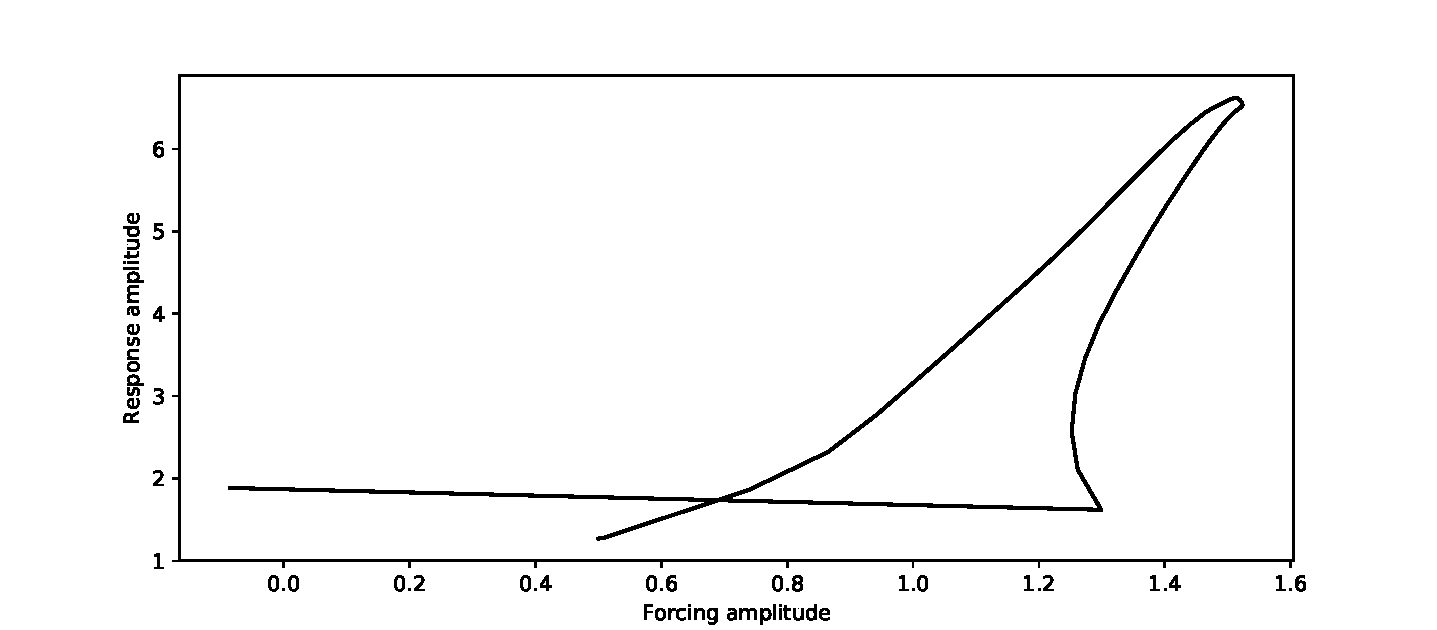
\includegraphics[width=.9\linewidth]{./5_knots_cbc.pdf}
\end{center}   

\begin{itemize}
\item Newton solvers don't converge on a solution

\item The solution curve becomes numerically unstable
\end{itemize}
\end{frame}
\end{document}
